\documentclass[12pt, a4paper]{article}
\setlength{\parindent}{0pt} 
\usepackage[utf8]{inputenc}
\usepackage[polish]{babel}
\addto\captionspolish{
  \renewcommand{\figurename}{Diagram}
}
\usepackage[T1]{fontenc}
\usepackage[colorlinks=true, linkcolor=black, urlcolor=blue]{hyperref}
\usepackage{pdfpages}
\usepackage[titletoc,title]{appendix}
\usepackage[nohyperlinks]{acronym}


\title{Master's Thesis on Big Data}
\author{Paweł Safuryn}
\date{2023}

\begin{document}


\includepdf[pages=-]{praca_koncowa_strona_tytulowa_BD.pdf}

% \begin{titlepage}
% \centering
% {\large Big Data - ed.14 (23L) - Projekt końcowy\par}
% {\huge\bfseries Master's Thesis on Big Data\par}
% \vspace{1.5cm}
% {\scshape\LARGE Politechnika Warszawska \par}
% \vspace{1.5cm}
% {\itshape Paweł Safuryn\par}
% \vfill
% Przedmiot ,,Projektowanie rozwiązań Big Data'' prowadzony przez \par
% mgr inż.~Damiana Warszawskiego

% \vfill

% % Bottom of the page
% {\large \today\par}
% \end{titlepage}

% \addcontentsline{toc}{section}{Streszczenie}
% \begin{abstract}
% This is where you write your abstract. It should briefly summarize the content of your thesis.
% \end{abstract}
% \newpage

\tableofcontents
\newpage

\section*{Akronimy}
\addcontentsline{toc}{section}{Akronimy}
\begin{acronym}
\acro{ATP}{Association of Tennis Professionals}
\acro{AWS}{Amazon Web Services}
\acro{CLI}{Command-line Interface}
\acro{MiB}{Mebibajt (1 048 576 bajtów)}
\acro{WTA}{Women's Tennis Association}
% Add more acronyms here...
\end{acronym}



\section{Wstęp}
% Wprowadzenie do problematyki pracy. Wstęp na zakończenie powinien zawierać cel pracy oraz zakres pracy. 
% Nie ma wymogu co do wyboru zestawu danych, niemniej, przyczyny wyboru powinny zostać opisane. Niezależnie od wielkości wybranego zbioru danych, analiza powinna być wykonana za pomocą narzędzi do przetwarzania Big Data.
% Proces Data Engineering/Science można podzielić w ogólności na kroki:
% 1. Zbieranie surowych danych
% 2. Przetwarzanie danych
% 3. Eksploracja danych
% 4. Czyszczenie danych
% 5. Modelowanie (opcjonalne)
% 6. Produkt oparty na danych (czyste dane, analiza, wyniki itp.)
% 7. Komunikacja wyników

% Zalinkuj Githuba z calym kodem włącznie z kodem ktory wygenerowal ten dokument.


\subsection{}
% Cos a tym jak  tenis   sie teraz zmienia i jest wiecej analytiki, profesjonalni graczce decduja sie miec data analysts w swoim zespole ale moga sobie na to pozwolic tylka  najbogatsi gracze - niedostepne dla nowych zawodnikow
% Jak analytika moze pomagac i komu - zawodnicy, przygotowania do meczu, do treningow (nad czm najlepiej pracowac), ocena silnych i slabch punktow swoich i przeciwnikow. Ale takze dane pomagaja narodowym organizacja tenisowym lepiej wylapywac talenty i alokowac pieniadze w rozwoj - w ktorego zawodnika inwestowac i jak (co trenowac). Innego rodzaju dane (social media, player popularity) sa uzywane zeby zwiekszac fan engagement (out of scoper)

% Opisz jakie dane  są ogólnie dostepne na rynku (to moze byy troche literature review):
% Np. samozwancze data scraping, pierwsze proby oficialnego API scheme od ITF, duzo crowdsourcowanych danych gdzie ludzie sami ogladaja mecze i zapisuja statystyki

\section{Przegląd literatury}

\section{Opis danych}

% Opisz dane od Jeffa - ATP i WTA
% Dokladny opis tego co tam jest i jak jest skonstruowane
% Czy unikalne ID gracza nachodza sie miedzy ATP i WTA? - tak - sa te same ID miedzy ATP i WTA
% Statystyki z Futuresow nie  maja bardziej szczegolowych statystyk tak jak mecze  ATP
% Wyjasnij roznice miedzy danymi - ATP matches, Futures, Challengers
% Opisz jak duze sa te  dane - okolo 400 MiB, nie jest  to klasyczne Big Data ze wzgledu na ograniczenie AWS Academy Learner Lab. Te dane zawsze moga rosnac i byc rozszerzone np. tagged video analysis do KAŻDEGO meczu ktory ma obraz wideo dostepny.

\section{Metodologia}

\subsection{Ustawienie środowiska}
\subsubsection{AWS Academy Learner Lab i AWS CLI}
Projekt wykonywany jest z użyciem AWS Academy Learner Lab [61569] i AWS CLI version 2. AWS CLI jest konfigurowane poprzez skopiowanie ustawień AWS Academy Learner Lab (dostępnych w "AWS Details") do  pliku:
\begin{verbatim}
~/.aws/credentials
\end{verbatim}

Opis architektury Big Data i indywidualnych technologii AWS wykorzystanych podczas projektu znajduje się w sekcji \ref{sec:aws_architecture}.

\subsubsection{Narzędzia używane lokalnie}
Poniżej znajduje się lista głównych narzędzi używanych lokalnie podczas projektu:
\begin{itemize}
    \item Python (wersja 3.9) --- główny język programowania używany do przetwarzania i analizy danych.
    \item Bash --- używany do automatyzacji zadań, głównie tych wykorzystujących AWS CLI.
    \item MacTeX i \LaTeX --- używane do napisania tej pracy końcowej.
    \item GitHub i Git --- kontrola wersji. Cały kod dostępny na repozytorium \href{https://github.com/safurynp/pw-big-data-final-project}{pw-big-data-final-project}.
    \item Miniconda --- zarządzanie środowiskiem wirtualnym oraz bibliotekami programistycznymi (np. do Pythona). Środowisko może być załadowane używając:
\begin{verbatim}
conda env create -f environment.yml
conda activate big-data-env
\end{verbatim}

\end{itemize}

\subsection{Architektura Big Data w AWS} \label{sec:aws_architecture}
Diagram \ref{fig:aws_architecture} przedstawia ogólny zarys architektury Big Data w AWS użytej w projekcie.
\begin{figure}[h]
    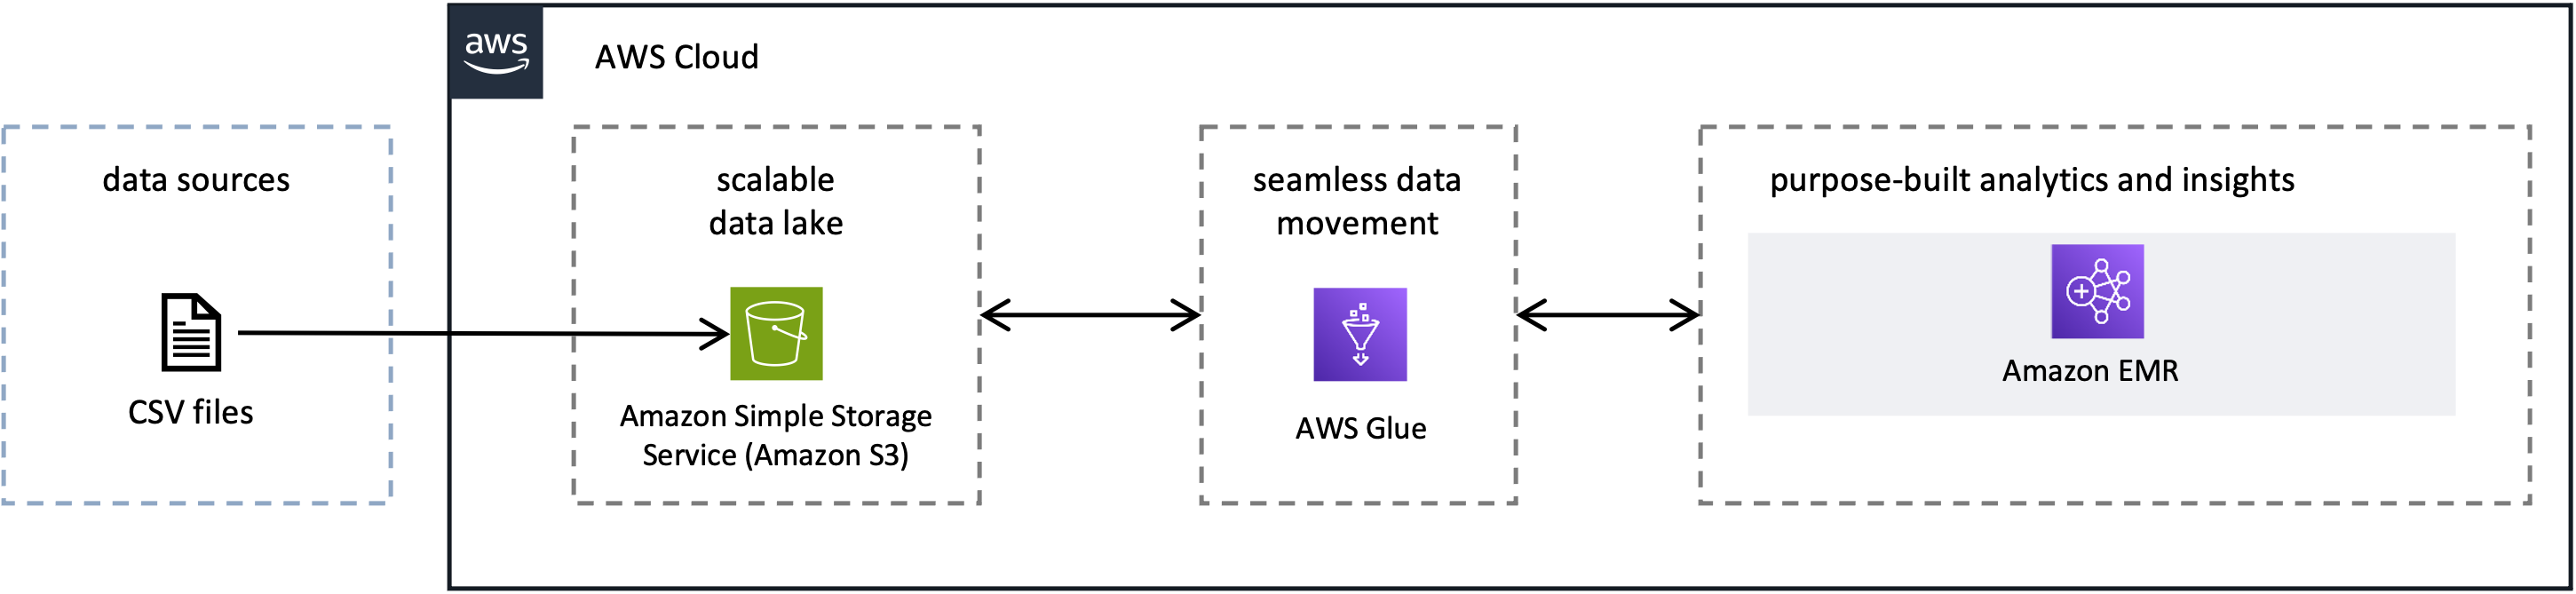
\includegraphics[width=\textwidth]{figures/aws_architecture.png}
    \caption{Architektura Big Data w AWS.}
    \label{fig:aws_architecture}
\end{figure}

Architektura ta składa się z następujących elementów:
\begin{enumerate}
    \item Surowych danych w formacie plików CSV.
    \item Amazon Single Storage Service (Amazon S3) używanego do przechowywania surowych danych oraz przetworzonych danych.
    \item 
\end{enumerate}

% Moze:
% 1. Jakis Pipeline zeby ladowal automatycznie dane z repo Jeffa do S3 bucketow
%  - moze sprawdzac regularnie czy jest nowy commit i wtedy aktualizowac wszystkie dane
% 2. Zrob jakies konrketne trasnformacje na tych danych (oczyszczanie, itd.)
% 3. Wizualizacje i analityka

\subsection{Zbieranie danych}
\subsubsection{Pozyskanie surowych danych}
Surowe tenisowe dane pozyskane są z dwóch repozytoriów na GitHubie Jeffa Sackmanna.
\begin{itemize}
    \item Dla profesjonalnego tenisa męskiego (ATP) \cite{tennis_atp}.
    \item Dla profesjonalnego tenisa żeńskiego (WTA) \cite{tennis_wta}.
\end{itemize}
Dane zostały pozyskane przez autora najprawdopodobniej (bazując na opisie repozytoriów) poprzez ekstrakcję danych (\textit{web scraping}) z Wikidata i oficjalnych stron organizacji ATP i WTA..
Dane są dostępne w formacie CSV. Dane dla ATP i WTA mają ten sam format i zawierają:
\begin{itemize}
    \item Statystyki z singlowych meczów tenisowych z głównego cyklu turniejów ATP i WTA (np. Wielkie Szlemy, ATP/WTA 1000). Dostępne są dla każdego roku od 1968 (początek ery Open) do 2023. Statystyki dla każdego roku są zawarte w osobnym pliku CSV.
    \item Statystyki z singlowych meczów tenisowych z etapów eliminacji oraz z niższych rangą turniejów ATP i WTA (np. Challengers, Futures). Te dostępne są od lat 1968/1978/1991 (w zależności od rodzaju turnieju) do 2023. Statystyki dla każdego roku są zawarte w osobnym pliku CSV.
    \item Lista graczy tenisa ziemnego, którzy grali w profesjonalnym turnieju ATP lub WTA wraz z podstawowymi informacjami na ich temat.
    \item Informacje o profesjonalnym rankingu ATP i WTA (aktualizowane co tydzień) od lat 70 do 2023. Statystyki dla każdej dekady i roku 2023 są zawarte w osobnym pliku CSV.
\end{itemize}
W sumie jest to 260 plików CSV o całkowitym rozmiarze 391,3 MiB. Repozytoria Jeffa Sackmanna na GitHubie zawierają również statystyki z meczów deblowych i amatorskich ale te zostały pominięte w tym projekcie. Bardziej szczegółowy opis surowych danych znajduje się w załączniku \ref{sec:raw_data_description}.

\subsubsection{Przesyłanie danych do chmury AWS}





% CSV files -> S3 bucket -> EMR Notebook
% Dodatkowo: CSV files -> AWS Lambda (commits) -> S3 bucket -> AWS Glue (co to robi?) -> AWS Athena (co to robi?) ->  EMR Notebook
% Ultimately, using AWS Transfer Family for uploading CSV files onto S3 provides a more robust, managed, and versatile solution compared to direct uploads, especially if you need to support multiple protocols, manage access control tightly, and monitor transfer activities closely.



\subsection{Przetwarzanie i czyszczenie danych}
% Moje zastosowanie nie wymaga przetwarzania strumieniowego - przetwarzanie wsadowe jest  wystarczajace poniewaz przetwarzam dane  juz zebrane i historyczne  do moich celow biznesowych. Dane sa przetwarzane jako zbior niezaleznie od czasu ich wygenerowania. Nie potrzebuje szybkiej reakcji na dane w czasie rzeczywistym (do tego  by bylo przetwarzanie strumieniowe).

% 1.  'hand' i 'ioc' kolumny  zmienione z object na kategoryczne
% W hand zmien 'U' na NaN (U oznacza Unknown). A to Ambidextreous (oburęczny)

\subsection{Eksploracja danych}
\subsection{Modelowanie matematyczne i analiza danych}
% Np. do pomocy zawodnikom  -  pokaz ktora nawierzchnia jest dla nich najlepsza a ktora najgorsza (pomaga ustawic treningi)
\subsection{Produkt oparty na danych i komunikacja wyników}

\section{Wyniki}

\section{Wnioski i zakończenie}
% Tu należy umieścić wnioski końcowe wynikające z realizacji celu pracy dyplomowej oraz podsumowanie uzyskanych efektów. 

% Co bym zrobil wiecej
% - wlasny scaper danych albo bezposrednie poloczenie z API (ale nie ma API na stronach WTA/ATP/ITF)


% - Przeanalizuj statystyki deblowe (robilem tylko singlowe)
% - Automatyczne  testowanie kodu - np. unit  testing

% - Adding AWS Transfer Family (not avaialbe in AWS Academy Learner Lab) to upload CSV files to S3.
%   Ultimately, using AWS Transfer Family for uploading CSV files onto S3 provides a more robust, managed, and versatile solution compared to direct uploads, especially if you need to support multiple protocols, manage access control tightly, and monitor transfer activities closely.
%   Altough I didn't deal with huge amounts of data there are around  400  MiB  (Mebibytes) and I'm uploding multiple CSV files. This takes over 20 minutes to upload. This is prone to errors and an AWS Transfer Family could provide a more robust solution.
% - I could alsouse AWS Lambda to react to new commits in the repo and then start the pipeline from the beginning. Uzyc AWS Lambda zeby reagowac na nowy commit w repo - gdy przybywa nowy plik CSV to rozpoczynam caly pipeline od nowa

% - Zrobic webowa aplikacje gdzie mozna filtrowac rozne tenisowe dane - nowy git commit moglby triggerowac caly pipeline konczacy sie deployowaniem tej aplikacji z nowymi danymi. Trenerzy, institycje tenisowy moglyby latwo przegladac te dane.




\nocite{*} % This line includes all references in the bibliography

\renewcommand{\refname}{Bibliografia}
\addcontentsline{toc}{section}{\refname}
\bibliographystyle{IEEEtran}
\bibliography{bibliography/references}

\begin{appendices}
\renewcommand{\appendixname}{Załącznik}  % Change the name to Polish

\section{Opis surowych danych} \label{sec:raw_data_description}

\end{appendices}

\end{document}